\chapter{Experimental results and discussion}

\section{Tabulated benchmarks}

\subsection{Experimental setup}

% Tabular benchmarks and statistical tests
In order to gain insight into the performance of the algorithms, first, we perform experiments on tabular benchmarks LCBench, FCNet, and NAS-Bench-201. The budget is limited by the number of epochs to 20 full evaluations. For example, all models in LCBench are trained for 50 epochs, so the total budget is 1000 epochs for all LCBench benchmarks. The reported metrics differ across datasets and benchmarks, so we convert all metrics to minimization and normalize the values into the range from 0 to 1 for each benchmark. We perform 30 repetitions for all benchmarks and algorithms and take the average. In accordance with the best practices for statistical comparison of algorithms across many datasets by Demšar~\cite{demvsar2006statistical}, we use the Friedman test to test the null hypothesis that all algorithms are equivalent. If the Friedman test rejects the null hypothesis, we follow up with the Wilcoxon signed-rank post-hoc test corrected with the Holm method to determine which algorithms perform differently. These tests are recommended because of several properties. They are non-parametric and have almost no assumptions on the data distribution. Since we cannot guarantee normality and homogeneity of variance of the results, it is safer not to use parametric tests like ANOVA.\@ The Wilcoxon test ranks the data internally, so the magnitude of values matters, but only to a limited extent, which is also desired.

% Algorithms
Because tabulated benchmarks are relatively cheap to evaluate, we can choose a wide array of algorithms for the comparison. We include several baseline model-less algorithms so that we see what results can be achieved without a surrogate model. Most of the model-based algorithms are based on the Gaussian process Bayesian optimization with the exception of DEHB.\@ \xxx{Maybe implement TPE-based, or RF-based model into Syne-tune as well?} We chose the following algorithms for the comparison:
\begin{itemize}
\item \textbf{Random search:} Random search serves the purpose of a baseline.
\item \textbf{Hyperband:} To see how much difference the synchronous early-stopping makes.
\item \textbf{ASHA:} Simple asynchronous early-stopping baseline.
\item \textbf{BOHB:} Popular model-based Hyperband algorithm.
\item \textbf{DEHB:} So that we have other models than Bayesian optimization.
\item \textbf{MOBSTER:} Asynchronous model-based baseline.
\item \textbf{Hyper-Tune:} Should be an improvement over the MOBSTER.
\item \textbf{DyHPO:} The most recent algorithm, even though we do not use the original deep kernel version, but normal Gaussian process is used.
\end{itemize}


% Library and metacentrum
We use the Syne-tune~\cite{salinas2022syne} library to perform the experiments. Computational resources were provided by the e-INFRA CZ project (ID:90254),
supported by the Ministry of Education, Youth and Sports of the Czech Republic.

\subsection{Results}
First, we show the aggregated results in Figure~\ref{ci:tabular}, which shows the average ranks of the algorithms across the 12 datasets from 3 tabulated benchmarks. The connecting bars signify that there is not a statistically significant difference between the algorithms. \xxx{With the Holm p-value correction there are almost no significant differences. LCBench has more datasets, but then the results would be biased towards the LCBench tasks and the tasks are easier.}

\begin{figure}[H]
    \centering
    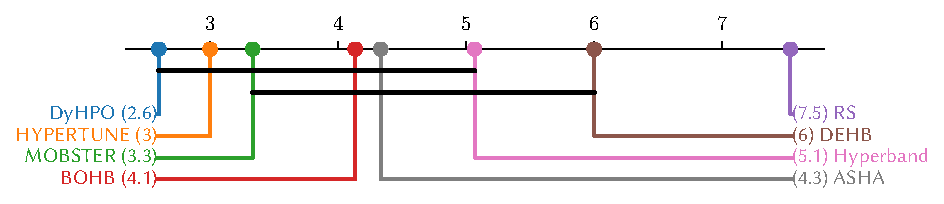
\includegraphics[scale=0.60]{./img/tabular_exp/cd_diagram.pdf}
    \caption{Critical difference diagram from tabular benchmarks at the maximal budget. Average ranks are shown on the x-axis.}
    \label{ci:tabular}
\end{figure}

Next, we illustrate the results of one benchmark in Figure~\ref{fig:parkinsons}. We provide the complete results in Appendix~\ref{ch:tabular}. We chose the FCNet Parkinsons dataset because it allows us to show several general traits and performance of the algorithms. It is often the case in our experiments that random search is clearly behind all other algorithms, but it is catching up as the budget increases. We can also notice the fixed schedule of the Hyperband. It takes nearly 10 full evaluations for the Hyperband to finish the first iteration (\xxx{or bracket?}) and to evaluate at least one configuration fully. We can also notice that in the first iteration, the model-less Hyperband performs similarly to the model-based extensions. The DEHB did not perform well in our experiments, it was often outperformed by model-less approaches. The performance of the most advanced methods was comparable. We cannot conclusively say that one is better than the other, as it often depends on the specific problem.

\begin{figure}[H]
    \centering
    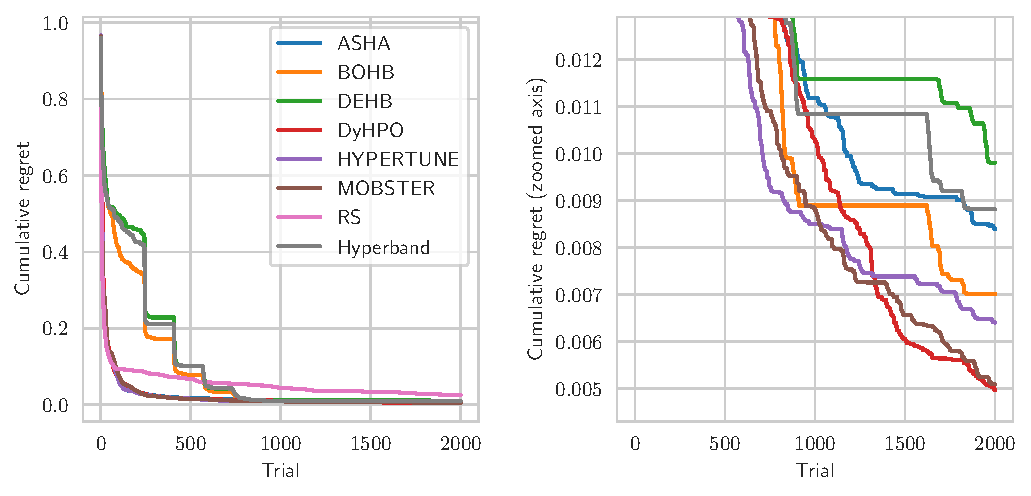
\includegraphics[scale=0.58]{img/tabular_exp/fcnet-parkinsons_plot.pdf}
    \caption{The averaged and normalized cumulative performance metric over 30 runs on the FCNet Parkinsons benchmark. On the right, we show the same results but zoomed in.}
    \label{fig:parkinsons}
\end{figure}


The key focus of this thesis is efficiency. A good way to measure efficiency is to compare the algorithms to Random Search and measure how much faster can they find a solution as good as the Random Search has found after spending the whole budget. We call it the speedup factor and present the results in Table~\ref{tab:speedup}. The reported speedup factor is averaged over all benchmarks and repetitions. We assume a speedup is greater than one, which was broken for one dataset, where the Random Search showed the best performance with a small margin. Because we do not have the data beyond the maximal budget, we have set the speedup factor to 1 in such cases.

\subfile{./tables/tab_results.tex}


In order to estimate the reliability and consistency of the methods, we provide the heatmap of variances in Figure~\ref{fig:heatmap}. \xxx{But it is hard to interpret the results. Especially where the Random Search is doing okay.}

\begin{figure}
    \centering
    \includegraphics[scale=0.6]{img/tabular_exp/variance_heatmap.pdf}
    \caption{The heatmap of variances of the best performance across the 30 repetitions. The variances are normalized for each benchmark.}
    \label{fig:heatmap}
\end{figure}


\section{Real benchmarks}


\subsection{Evaluation}

% What resource are we using
First, we need to specify how to measure the used resources and limit the total budget. We can measure either the wall-clock time, or the number of epochs. Measuring function evaluations does not make sense because of multi-fidelity evaluations --- each evaluation could be at a different budget. The wall-clock time is the quantity that matters in real-world applications, but the number of epochs is easier to work with, especially when the experiments are run at a heterogeneous computer cluster. It comes at the cost of neglecting the overhead of the hyperparameter optimization algorithms and gives a small advantage to the more computationally heavy algorithms. On the other hand, it allows for a direct comparison of sample efficiency and the overhead of a hyperparameter optimization algorithm is negligible in most scenarios encountered when tuning hyperparameters of deep neural networks, as we will show.

% Single dataset
We chose to evaluate the performance at 20 full function evaluations and 10 full evaluations. We use the Kruskal test to determine whether there is any difference at all, and then we use the Mann-Whitney rank sum test to determine pairwise differences.


\subsection{Datasets and models}
We will run the tests on the chosen tabular benchmarks first. For real-world examples, we can compare the algorithms on image data (CIFAR10, SVHN) and with a simple CNN model, or xResNet model.

We also tested the tuning algorithms on a medical dataset PTB-XL. PTB-XL is a collection of 21837 clinical 12-lead ECGs of 10 second length annotated by up to two cardiologists with ECG statements. In the multilabel classification task, the goal is to assign 1 or more of the 5 diagnostic superclasses. We can perform an experiment using a LSTM RNN, 1d-CNN, or 1d xResNet architecture.


\subsection{Experimental Setup}


% I could split this chapter into two.


\subsection{CIFAR10 - demo}

Probably the most widely used image classification dataset is the CIFAR-10. We use it to evaluate the performance of Random Search, DEHB, Optuna and DyHPO hyperparameter optimization algorithms \xxx{(not the final set of algorithms)}. The optimization was rerun 5 times for each algorithm with different seed \xxx{but this seems to be too little, the means are not significantly different}. The optimization problem consisted of six hyperparameters, three float and three integer. We used AdamW optimizer. Learning rate and the final value of cosine decay $\eta_{min}$ were optimized. The neural network architecture consists of sequential convolutional layers with batch normalization. We optimize the number of convolutional layers and the number of filters. Then the fully connected layer follows and we optimize its size. The hyperparameters and their domains are summarized in the Table~\ref{tc10}.

\begin{table}[H]
    \centering
    \begin{tabular}{cc}
        \textbf{Hyperparameter} & \textbf{Values} \\ \midrule
        Learning rate & $\{1\mathrm{e}{-4}, 1\mathrm{e}{-1}\}$ \\
        $\eta_{min}$ & $\{1\mathrm{e}{-5}, 0.99\}$ \\
        Dropout & $\{0.0, 1.0\}$ \\
        FC neurons & $\{8, 128\}$ \\
        Channels multiplier & $\{1, 8\}$ \\
        Conv layers & $\{1, 4\}$ \\
    \end{tabular}
    \caption{CIFAR-10 HPO optimization search space.}
    \label{tc10}
\end{table}

The network is trained for up to 70 epochs. The budget for the hyperparameter optimization is 17 full evaluations, which is equal to 1190 epochs. We compare the algorithms in classification accuracy on the validation set. We use the trial number on the x-axis, which neglects the cost of the hyperparameter optimization algorithm.

\begin{figure}[H]
    \centering
    \includegraphics[scale=0.64]{./img/cifar_exp_plot.pdf}
    \caption{CIFAR-10 comparison of the best cumulative accuracy, 17 full evaluations (1190 epochs)}
    %\label{}
\end{figure}

The following plots are evaluated after 350 training epochs \xxx{because that is where the difference is the largest; so that we can test if the results will be statistically significant, or if we need more repetitions}.

\begin{figure}[H]
    \centering
    \includegraphics[scale=0.74]{./img/cifar_exp_boxplot.pdf}
    \caption{CIFAR-10 boxplot after 350 epochs.}
    %\label{}
\end{figure}

%\xxx{I wanted to use critical difference diagrams for the visualization of performance and statistical analysis because I think they are intuitive and easily readable, but I'm not sure if I can do it even for unpaired experiements. CD diagrams rely on computing the rank of the methods --- comparing the results of different runs to each other.} We used the Mann-Whitney rank sum test for the post-hoc analysis of the results with the significance level $\alpha=0.05$ adjusted with the Holm's method.

% \begin{figure}[H]
%     \centering
%     \includegraphics[scale=0.74]{./img/cifar_exp_cd_ranks.pdf}
%     \caption{CIFAR-10 critical difference diagram}
%     %\label{}
% \end{figure}
\subsection{SVHN}


\section{Discussion}
